%==============================================================================
%  DigiRadio -- Technical Reference Manual
%  DAB+/FM Bluetooth Receiver with SigmaDSP Audio Processing
%  (c) Michele Bigi -- Open Source Hardware
%==============================================================================
\documentclass[11pt,a4paper]{report}

\usepackage[utf8]{inputenc}
\usepackage[T1]{fontenc}
\usepackage[margin=2.4cm]{geometry}
\usepackage{graphicx}
\usepackage{xcolor}
\usepackage{booktabs}
\usepackage{array}
\usepackage{tabularx}
\usepackage{longtable}
\usepackage{titlesec}
\usepackage{fancyhdr}
\usepackage{enumitem}
\usepackage{listings}
\usepackage{tikz}
\usetikzlibrary{shapes.geometric,arrows.meta,positioning,calc,fit,backgrounds}
\usepackage[most]{tcolorbox}
\usepackage[hidelinks,colorlinks=true,linkcolor=brandblue,urlcolor=brandblue,citecolor=brandblue]{hyperref}

\definecolor{brandblue}{HTML}{1F4E78}
\definecolor{brandcyan}{HTML}{2E86AB}
\definecolor{brandgrey}{HTML}{4D4D4D}
\definecolor{lightgrey}{HTML}{F0F0F0}
\definecolor{rfcol}{HTML}{C0392B}
\definecolor{dspcol}{HTML}{27AE60}
\definecolor{btcol}{HTML}{2E86AB}
\definecolor{mcucol}{HTML}{8E44AD}
\definecolor{pwrcol}{HTML}{E67E22}
\definecolor{gndcol}{HTML}{7F8C8D}

\titleformat{\chapter}[display]
  {\normalfont\huge\bfseries\color{brandblue}}
  {\chaptertitlename\ \thechapter}{10pt}{\Huge}
\titleformat{\section}
  {\normalfont\Large\bfseries\color{brandblue}}{\thesection}{1em}{}
\titleformat{\subsection}
  {\normalfont\large\bfseries\color{brandcyan}}{\thesubsection}{1em}{}

\pagestyle{fancy}
\fancyhf{}
\renewcommand{\headrulewidth}{0.4pt}
\fancyhead[L]{\small\color{brandgrey}DigiRadio}
\fancyhead[R]{\small\color{brandgrey}Technical Reference Manual}
\fancyfoot[C]{\thepage}

\newtcolorbox{designbox}[1][]{colback=brandblue!5,colframe=brandblue,coltitle=white,
  fonttitle=\bfseries,title={Design Decision},boxrule=0.8pt,arc=2pt,left=6pt,right=6pt,top=4pt,bottom=4pt,#1}
\newtcolorbox{notebox}[1][]{colback=brandcyan!6,colframe=brandcyan,coltitle=white,
  fonttitle=\bfseries,title={Note},boxrule=0.8pt,arc=2pt,left=6pt,right=6pt,top=4pt,bottom=4pt,#1}
\newtcolorbox{warnbox}[1][]{colback=rfcol!6,colframe=rfcol,coltitle=white,
  fonttitle=\bfseries,title={Important},boxrule=0.8pt,arc=2pt,left=6pt,right=6pt,top=4pt,bottom=4pt,#1}

\lstset{basicstyle=\ttfamily\small,breaklines=true,frame=single,
  rulecolor=\color{brandgrey},backgroundcolor=\color{lightgrey},
  keywordstyle=\color{brandblue}\bfseries,commentstyle=\color{dspcol}}

\newcommand{\version}{v1.0 (pre-prototype)}
\newcommand{\ic}[1]{\texttt{#1}}

\begin{document}

%----------------------------------- Title page -------------------------------
\begin{titlepage}
\centering
\vspace*{2.0cm}
{\color{brandblue}\rule{\textwidth}{2pt}}\\[0.6cm]
{\Huge\bfseries\color{brandblue} DigiRadio}\\[0.35cm]
{\LARGE DAB+/FM Bluetooth Receiver}\\[0.15cm]
{\LARGE with SigmaDSP Audio Processing}\\[0.5cm]
{\color{brandblue}\rule{\textwidth}{2pt}}\\[1.0cm]
{\Large Technical Reference Manual}\\[0.3cm]
{\large \version}\\[1.4cm]

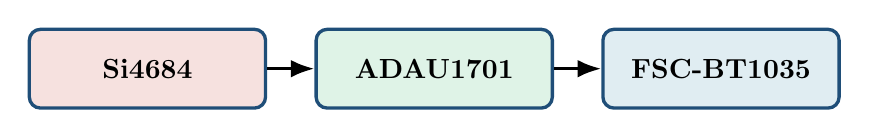
\begin{tikzpicture}[scale=1]
  \node[draw=brandblue,very thick,rounded corners,minimum width=3.0cm,minimum height=1.0cm,fill=rfcol!15]  (rf)  {\bfseries Si4684};
  \node[draw=brandblue,very thick,rounded corners,minimum width=3.0cm,minimum height=1.0cm,fill=dspcol!15,right=0.6cm of rf] (dsp) {\bfseries ADAU1701};
  \node[draw=brandblue,very thick,rounded corners,minimum width=3.0cm,minimum height=1.0cm,fill=btcol!15,right=0.6cm of dsp] (bt) {\bfseries FSC-BT1035};
  \draw[-{Latex[length=3mm]},very thick] (rf)--(dsp);
  \draw[-{Latex[length=3mm]},very thick] (dsp)--(bt);
\end{tikzpicture}\\[0.8cm]

\IfFileExists{Hardware/3d/render.png}{\includegraphics[width=0.72\textwidth]{Hardware/3d/render.png}\\[0.4cm]}{}

\vfill
{\large Michele Bigi}\\[0.2cm]
{\normalsize Open-Source Hardware Project}\\[0.2cm]
{\small Manufactured with PCBWay --- 6-layer, impedance-controlled}\\[0.8cm]
{\small\itshape Licensed under CERN-OHL-S (hardware) and MIT (firmware)}
\end{titlepage}

\tableofcontents
\thispagestyle{fancy}

%==============================================================================
\chapter{Overview}
%==============================================================================
\section{Introduction}
DigiRadio is an open-source digital radio receiver that combines terrestrial
broadcast reception (\textbf{DAB+ / DAB / FM}) with a programmable audio-processing
stage and high-quality \textbf{Bluetooth} audio output. Incoming broadcast audio is
decoded by a Silicon Labs \ic{Si4684} digital-radio receiver, processed by an Analog
Devices \ic{ADAU1701} SigmaDSP (equalisation, mixing, level control), and transmitted
over Bluetooth by a Qualcomm QCC3056-based \ic{FSC-BT1035} module supporting the
\textbf{aptX Adaptive} codec. An Espressif \ic{ESP32-S3} acts as the host controller,
orchestrating the three subsystems and providing Wi-Fi/BLE connectivity and a USB
service interface. The tuner$\rightarrow$DSP$\rightarrow$Bluetooth path is fully
digital (I\textsuperscript{2}S, 48\,kHz / 24-bit).

\IfFileExists{Hardware/3d/render.png}{%
\begin{figure}[h]\centering
\includegraphics[width=0.85\textwidth]{Hardware/3d/render.png}
\caption{DigiRadio 6-layer PCB (3D render), 50\,$\times$\,90\,mm.}\end{figure}}{}

\section{Key Features}
\begin{itemize}[leftmargin=1.4em,itemsep=2pt]
  \item DAB+ / DAB / FM reception (Si4684) via external whip antenna (SMA).
  \item Fully digital audio path (I\textsuperscript{2}S, 48\,kHz / 24-bit).
  \item Programmable audio processing on the ADAU1701 SigmaDSP.
  \item Bluetooth 5.2 output with aptX / aptX HD / \textbf{aptX Adaptive}.
  \item ESP32-S3 host with native USB, Wi-Fi and BLE.
  \item USB-C powered; 3.3\,V main rail + low-noise 1.8\,V for the tuner.
  \item 6-layer impedance-controlled PCB, 50\,$\times$\,90\,mm, two ground planes.
  \item Three antennas (ESP32 2.4\,GHz, BT1035 2.4\,GHz, FM/DAB SMA) with keep-outs.
\end{itemize}

\begin{designbox}
The design goal was \emph{sound quality first} for the wireless link. Because the
final DAC lives in the Bluetooth sink, the codec is the single most important quality
factor in the chain. The QCC3056/aptX~Adaptive path was chosen over cheaper
SBC/AAC-only modules, and the whole tuner$\rightarrow$DSP$\rightarrow$BT path is kept
digital to avoid any avoidable A/D--D/A conversion.
\end{designbox}

%==============================================================================
\chapter{System Architecture}
%==============================================================================
\section{Signal Chain}
The audio signal flows entirely in the digital domain from tuner to Bluetooth
module (Figure~\ref{fig:chain}).

\begin{figure}[h]\centering
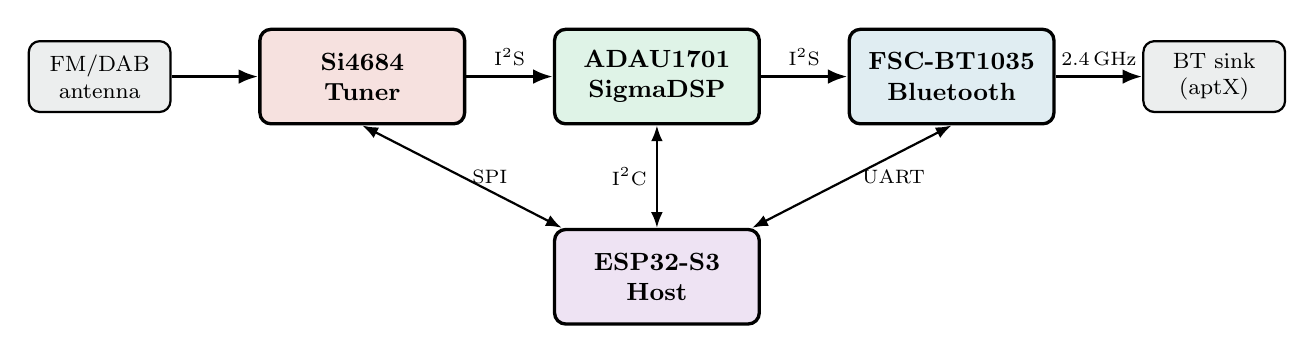
\begin{tikzpicture}[node distance=1.0cm and 1.1cm,
  block/.style={draw,very thick,rounded corners,minimum width=2.6cm,minimum height=1.2cm,align=center,font=\small\bfseries},
  ant/.style={draw,thick,rounded corners,minimum width=1.8cm,minimum height=0.9cm,align=center,font=\footnotesize,fill=gndcol!15},
  arr/.style={-{Latex[length=2.5mm]},very thick}]
  \node[ant] (fmant) {FM/DAB\\antenna};
  \node[block,fill=rfcol!15,right=of fmant] (rf) {Si4684\\Tuner};
  \node[block,fill=dspcol!15,right=of rf]   (dsp) {ADAU1701\\SigmaDSP};
  \node[block,fill=btcol!15,right=of dsp]   (bt)  {FSC-BT1035\\Bluetooth};
  \node[ant,right=of bt] (btant) {BT sink\\(aptX)};
  \draw[arr] (fmant)--(rf);
  \draw[arr] (rf)--node[above,font=\scriptsize]{I\textsuperscript{2}S}(dsp);
  \draw[arr] (dsp)--node[above,font=\scriptsize]{I\textsuperscript{2}S}(bt);
  \draw[arr] (bt)--node[above,font=\scriptsize]{2.4\,GHz}(btant);
  \node[block,fill=mcucol!15,below=1.3cm of dsp] (mcu) {ESP32-S3\\Host};
  \draw[{Latex[length=2mm]}-{Latex[length=2mm]},thick] (mcu)--node[right,font=\scriptsize]{SPI}(rf.south);
  \draw[{Latex[length=2mm]}-{Latex[length=2mm]},thick] (mcu)--node[left,font=\scriptsize]{I\textsuperscript{2}C}(dsp);
  \draw[{Latex[length=2mm]}-{Latex[length=2mm]},thick] (mcu)--node[right,font=\scriptsize]{UART}(bt.south);
\end{tikzpicture}
\caption{Signal chain. Audio (top) stays digital end-to-end; the ESP32-S3 host
(bottom) controls each subsystem over its own bus.}\label{fig:chain}
\end{figure}

\begin{notebox}
The ESP32-S3 can inject its own audio stream (e.g.\ Wi-Fi internet radio or prompts)
into the DSP over a second I\textsuperscript{2}S input, letting the DSP mix broadcast
and network audio before the Bluetooth stage.
\end{notebox}

\section{Clock Architecture}
The I\textsuperscript{2}S bus is driven by a single master. The ADAU1701 is the
I\textsuperscript{2}S \textbf{master}, generating BCLK and LRCLK from its 12.288\,MHz
crystal (12.288\,MHz\,/\,256 = 48\,kHz). The Si4684 and FSC-BT1035 are
I\textsuperscript{2}S slaves. The Si4684 keeps its own independent 19.2\,MHz reference
crystal for RF synthesis.

\begin{designbox}
The ADAU1701 was made I\textsuperscript{2}S master because it already carries a
12.288\,MHz crystal that divides cleanly to 48\,kHz ($\times$256). Making the BT
module master would have forced the DSP PLL to lock to an incoming LRCLK of possibly
44.1\,kHz, introducing a sample-rate mismatch (the ADAU1701 has no ASRC). With the
DSP as master, both tuner and BT module follow its clean 48\,kHz.
\end{designbox}

\section{Power Tree}
The board is powered from USB-C (5\,V). A buck converter generates the 3.3\,V rail;
a low-noise LDO derives the 1.8\,V rail required by the Si4684 analogue and memory
supplies (Figure~\ref{fig:power}).

\begin{figure}[h]\centering
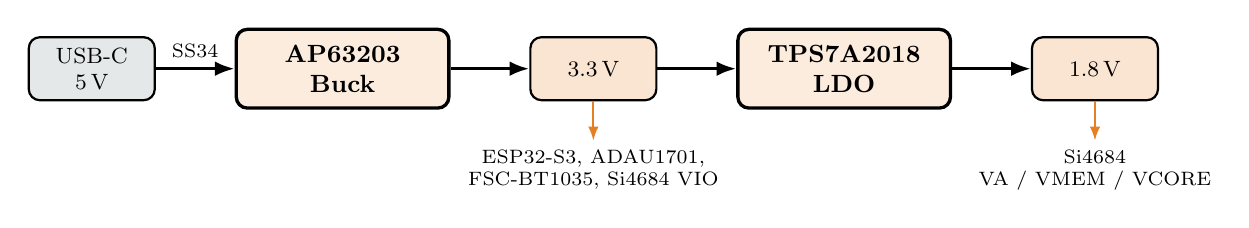
\begin{tikzpicture}[
  block/.style={draw,very thick,rounded corners,minimum width=2.7cm,minimum height=1.0cm,align=center,font=\small\bfseries},
  rail/.style={draw,thick,rounded corners,minimum width=1.6cm,minimum height=0.8cm,align=center,font=\footnotesize,fill=pwrcol!20},
  arr/.style={-{Latex[length=2.5mm]},very thick}]
  \node[rail,fill=gndcol!20] (usb) {USB-C\\5\,V};
  \node[block,fill=pwrcol!15,right=1.0cm of usb] (buck) {AP63203\\Buck};
  \node[rail,right=1.0cm of buck] (r33) {3.3\,V};
  \node[block,fill=pwrcol!15,right=1.0cm of r33] (ldo) {TPS7A2018\\LDO};
  \node[rail,right=1.0cm of ldo] (r18) {1.8\,V};
  \draw[arr] (usb)--node[above,font=\scriptsize]{SS34}(buck);
  \draw[arr] (buck)--(r33); \draw[arr] (r33)--(ldo); \draw[arr] (ldo)--(r18);
  \node[font=\scriptsize,below=0.5cm of r33,align=center] (c33){ESP32-S3, ADAU1701,\\FSC-BT1035, Si4684 VIO};
  \node[font=\scriptsize,below=0.5cm of r18,align=center] (c18){Si4684\\VA / VMEM / VCORE};
  \draw[-{Latex[length=1.8mm]},thick,pwrcol] (r33)--(c33);
  \draw[-{Latex[length=1.8mm]},thick,pwrcol] (r18)--(c18);
\end{tikzpicture}
\caption{Power tree. A single series Schottky (SS34) protects the USB input; the buck
feeds all 3.3\,V loads, and the LDO provides the quiet 1.8\,V rail for the tuner.}
\label{fig:power}
\end{figure}

\begin{warnbox}
The Si4684 requires 1.8\,V (not 3.3\,V) on \ic{VA}, \ic{VMEM} and \ic{VCORE}; only
\ic{VIO} may be 1.8--3.6\,V and is set to 3.3\,V here so that SPI and
I\textsuperscript{2}S logic levels match the ESP32 and DSP domains.
\end{warnbox}

%==============================================================================
\chapter{Functional Blocks}
%==============================================================================
\section{RF Front-End --- Si4684 Digital Radio Receiver}
The \ic{Si4684-A10-GM} (QFN-48) receives FM, DAB and DAB+ from an external whip
antenna through an SMA edge connector. The design follows Silicon Labs application
note \textbf{AN851} for the schematic and layout of the RF input and supply bypassing.

\subsection{Supplies and Sequencing}
\ic{VA}, \ic{VMEM} and \ic{VCORE} run from the 1.8\,V rail; \ic{VIO} runs from 3.3\,V
to match the host logic. \ic{SMODE} is tied low to select the SPI control bus, over
which the ESP32-S3 loads the tuner firmware/patch image at boot. \ic{RSTB} is held
low during supply ramp and released by the host only after both rails are stable.

\begin{warnbox}
During the SPI firmware download the chip-select (\ic{SSB}) must be held low for the
entire transaction --- it must not toggle between bytes. On the ESP32-S3, \ic{SSB} is
therefore driven as a software-controlled GPIO, not by the SPI peripheral's automatic
chip-select.
\end{warnbox}

\subsection{Supply Bypassing (AN851)}
Each supply pin (\ic{VA}, \ic{VMEM}, \ic{VCORE}, \ic{VIO}) carries a decoupling
triplet of 8.2\,pF (C0G), 2.2\,nF and 1\,\textmu F. Per AN851 these bypass capacitors
return to the internal bypass nodes \ic{DBYP} / \ic{ABYP}, \emph{not} to the general
ground plane; \ic{DBYP} and \ic{ABYP} are internal-regulator/return nodes and are not
tied to GND.

\begin{designbox}
This is the single most non-obvious detail of the Si468x. Applying the generic
``cap-to-ground'' decoupling rule here would be wrong: AN851 explicitly routes the
supply bypass capacitors to \ic{DBYP}/\ic{ABYP} to keep the receiver's reference
quiet. On the PCB each triplet is placed against its own pin, smallest value nearest
the pin, with the return via immediately after the capacitor.
\end{designbox}

\subsection{RF Matching and Protection}
The FM/DAB matching network (whip-antenna topology) comprises a 33\,pF DC-blocking
capacitor, an 18\,nH series inductor, a 2.7\,pF shunt (C0G), and 120\,nH / 22\,nH
tuning inductors into \ic{VHFI}/\ic{VHFSW}. A \ic{BAV99} dual diode provides
bidirectional ESD clamping: its common node sits on the RF line and both ends return
to ground, presenting the minimum shunt capacitance to the antenna.

\subsection{Reference Crystal}
A 19.2\,MHz crystal (10\,pF CL) with two 12\,pF C0G load capacitors provides the RF
reference. The crystal and its load caps are placed with a minimal loop against
\ic{XTALI}/\ic{XTALO}, guarded by ground and with an unbroken ground plane beneath.

\section{Audio DSP --- ADAU1701 SigmaDSP}
The \ic{ADAU1701JSTZ-RL} (LQFP-48) performs equalisation, mixing and level control.
It receives audio from the Si4684 (\ic{SDATA\_IN0}) and from the ESP32-S3
(\ic{SDATA\_IN1}), and outputs to the Bluetooth module (\ic{SDATA\_OUT0}).

\subsection{Clocking and I\textsuperscript{2}S Role}
The DSP is the I\textsuperscript{2}S master, clocked by a 12.288\,MHz crystal (two
22\,pF C0G load caps). \ic{PLL\_MODE0} and \ic{PLL\_MODE1} are both tied low for the
256\,$\times$\,fs ratio (12.288\,MHz / 48\,kHz = 256). \ic{VDRIVE} and \ic{IOVDD} are
at 3.3\,V so the digital outputs match the host logic. The PLL loop filter uses
475\,$\Omega$ / 3.3\,nF / 56\,nF per the datasheet.

\subsection{Program Loading}
The design uses the \textbf{host-load} model: \ic{SELFBOOT} is tied low, and the
ESP32-S3 writes the compiled SigmaStudio program into the DSP RAM over
I\textsuperscript{2}C at boot (halt core, write program/parameter RAM, restart). The
on-board self-boot EEPROM is an optional (unpopulated) footprint.

\begin{designbox}
Two decisions here came out of design review. First, host-load was chosen over
self-boot so the ESP32 is the sole I\textsuperscript{2}C master and also controls the
DSP at runtime --- eliminating the two-master contention that self-boot would create.
Second, an early revision wired the DSP control port only to its self-boot EEPROM and
\emph{not} to the system I\textsuperscript{2}C bus; that would have left the host
unable to change volume/EQ at runtime. The port is now on the shared system bus.
\end{designbox}

\subsection{Control Interface}
The DSP control port sits on the system I\textsuperscript{2}C bus (2.2\,k$\Omega$
pull-ups). \ic{CLATCH/WP} is tied to a defined level for I\textsuperscript{2}C mode;
\ic{ADDR0}/\ic{ADDR1} set the slave address. The reset line is driven by the host
(GPIO47) with a 10\,k$\Omega$ pull-up and a small POR capacitor.

\section{Bluetooth --- FSC-BT1035 (QCC3056)}
The \ic{FSC-BT1035} is a Bluetooth 5.2 audio module built on the Qualcomm QCC3056,
supporting A2DP/AVRCP/HFP and the aptX / aptX HD / \textbf{aptX Adaptive} codecs. In
DigiRadio it operates as an \textbf{A2DP source}, taking the processed I\textsuperscript{2}S
stream from the DSP and transmitting it to a Bluetooth sink.

\begin{itemize}[leftmargin=1.4em,itemsep=2pt]
  \item \textbf{I\textsuperscript{2}S slave:} \ic{PCM\_CLK}=BCLK, \ic{PCM\_SYNC}=LRCLK,
        \ic{PCM\_IN}=\ic{SDATA\_OUT0} from the DSP.
  \item \textbf{Power-on:} \ic{SYS\_CTRL} (host GPIO15, pull-down) asserts to power the
        module on; \ic{RESET} (host GPIO17) relies on the module's internal pull-up.
  \item \textbf{Control:} UART with the Feasycom ASCII command set (4-wire, flow control).
  \item \textbf{Supplies:} \ic{VBAT\_IN} = 3.3\,V, \ic{VDD\_IO} = 3.3\,V,
        \ic{1.8V\_OUT} bypassed only.
  \item \textbf{Firmware/role:} requires the Audio-Transceiver (source-capable)
        firmware in Host mode.
\end{itemize}

\begin{notebox}
The FSC-BT1035 is MSL-3 rated and must be baked before reflow. The PCB footprint
uses the pin-compatible BT806 land pattern.
\end{notebox}

\section{Host --- ESP32-S3-WROOM-1}
The \ic{ESP32-S3-WROOM-1-N16} host provides Wi-Fi, BLE, native USB and control of all
three subsystems. Native USB (GPIO19/20) handles programming and console, freeing
UART0 for a system-monitor header (CN1). UART1 (with flow control) drives the
FSC-BT1035. SPI controls the Si4684; the system I\textsuperscript{2}C controls the DSP
and MAC EEPROM. Dedicated GPIOs drive the DSP reset (GPIO47), the BT \ic{SYS\_CTRL}
(GPIO15) and the BT \ic{RESET} (GPIO17).

\section{Power Stage}
An \ic{AP63203WU-7} synchronous buck (fixed 3.3\,V, \ic{EN}=\ic{VIN}, 100\,nF
bootstrap, 4.7\,\textmu H inductor, 22\,\textmu F output) generates the main rail from
the USB-C input protected by a single \ic{SS34} Schottky. A \ic{TPS7A2018} low-noise
LDO (\ic{EN}=3.3\,V) derives the 1.8\,V rail. USB ESD is handled by an \ic{SRV05-4}
at the connector.

%==============================================================================
\chapter{PCB Design}
%==============================================================================
\section{Layer Stack-up}
DigiRadio uses a 6-layer stack with two dedicated ground planes, so that sensitive RF
and clock nets on the top layer reference a solid, uninterrupted ground plane
immediately beneath (Figure~\ref{fig:stack}).

\begin{figure}[h]\centering
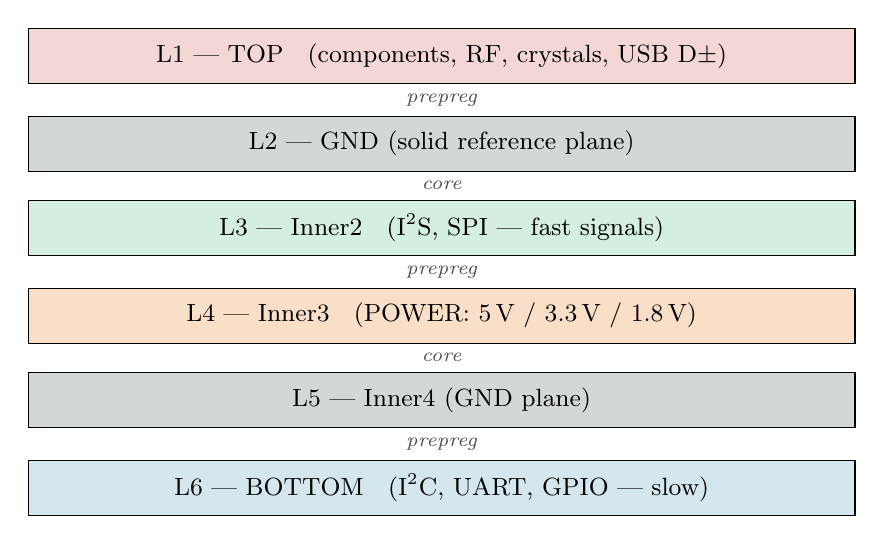
\begin{tikzpicture}[
  lay/.style={draw,minimum width=10.5cm,minimum height=0.7cm,font=\small,align=center},
  die/.style={minimum width=10.5cm,minimum height=0.3cm,font=\scriptsize\itshape,align=center,text=brandgrey}]
  \node[lay,fill=rfcol!20]  (l1) {L1 --- TOP \; (components, RF, crystals, USB D$\pm$)};
  \node[die,below=0pt of l1] (p12) {prepreg}; \node[lay,fill=gndcol!35,below=0pt of p12] (l2) {L2 --- GND (solid reference plane)};
  \node[die,below=0pt of l2] (c23) {core}; \node[lay,fill=dspcol!20,below=0pt of c23] (l3) {L3 --- Inner2 \; (I\textsuperscript{2}S, SPI --- fast signals)};
  \node[die,below=0pt of l3] (p34) {prepreg}; \node[lay,fill=pwrcol!25,below=0pt of p34] (l4) {L4 --- Inner3 \; (POWER: 5\,V / 3.3\,V / 1.8\,V)};
  \node[die,below=0pt of l4] (c45) {core}; \node[lay,fill=gndcol!35,below=0pt of c45] (l5) {L5 --- Inner4 (GND plane)};
  \node[die,below=0pt of l5] (p56) {prepreg}; \node[lay,fill=btcol!20,below=0pt of p56] (l6) {L6 --- BOTTOM \; (I\textsuperscript{2}C, UART, GPIO --- slow)};
\end{tikzpicture}
\caption{6-layer stack-up. Fast signals (L3) are sandwiched between GND (L2) and POWER
(L4); slow signals live on the bottom, referenced to the second GND plane (L5).}
\label{fig:stack}
\end{figure}

\begin{designbox}
The stack is built around signal integrity, not routing convenience. The USB
differential pair is routed on \textbf{TOP}, referenced to the L2 ground plane, where
90\,$\Omega$ differential impedance is achievable at manufacturable trace widths
(6\,mil trace / 8\,mil gap). Routing it on an inner layer through the thicker
core would have required non-manufacturable trace widths.
\end{designbox}

\section{Controlled Impedance}
\begin{center}\begin{tabularx}{\textwidth}{@{}l l l X@{}}
\toprule
\textbf{Net} & \textbf{Layer} & \textbf{Target} & \textbf{Geometry (PCBWay 6-layer)}\\
\midrule
USB D+/D-- & TOP / ref L2 & 90\,$\Omega$ diff & 6\,mil trace, 8\,mil gap \\
FM/DAB RF  & TOP / ref L2 & microstrip     & short, in-line, no vias in path \\
I\textsuperscript{2}S / SPI & Inner2 & --- (digital) & 6\,mil, GND-referenced \\
\bottomrule
\end{tabularx}\end{center}

\section{Plane Continuity and Keep-outs}
The L2 ground plane is kept solid and unbroken under the RF trace, the two crystals
and the USB pair; verification confirmed no plane splits or via ``slots'' in these
regions. Three antenna zones are cleared of copper on \emph{all} layers: the ESP32-S3
module antenna, the FSC-BT1035 module antenna, and the FM/DAB SMA trace. The two
2.4\,GHz antennas (ESP32, BT1035) are placed diagonally to maximise separation.

%==============================================================================
\chapter{Interfaces and Bus Map}
%==============================================================================
\section{I\textsuperscript{2}S Topology}
The DSP is master; the Si4684 and FSC-BT1035 are slaves. BCLK and LRCLK are single
nets shared by all I\textsuperscript{2}S devices; each clock reaches every device that
uses it (including both DSP serial ports).
\begin{center}\begin{tabularx}{\textwidth}{@{}l X@{}}
\toprule \textbf{Signal} & \textbf{Path} \\ \midrule
BCLK / LRCLK & ADAU1701 (master) $\rightarrow$ Si4684, FSC-BT1035, ESP32 \\
SDATA\_IN0 & Si4684 $\rightarrow$ ADAU1701 \\
SDATA\_IN1 & ESP32-S3 $\rightarrow$ ADAU1701 \\
SDATA\_OUT0 & ADAU1701 $\rightarrow$ FSC-BT1035 \\
\bottomrule \end{tabularx}\end{center}

\section{I\textsuperscript{2}C Address Map}
A single system I\textsuperscript{2}C bus (2.2\,k$\Omega$ pull-ups to 3.3\,V) hosts the
DSP and the MAC EEPROM; the self-boot EEPROM is a DNP option.
\begin{center}\begin{tabularx}{\textwidth}{@{}l l X@{}}
\toprule \textbf{Device} & \textbf{Address} & \textbf{Role} \\ \midrule
ADAU1701 & 0x68 (ADDR=00) & DSP control \\
24AA025E48 & 0x52 & MAC / EUI-48 EEPROM \\
24LC256 (DNP) & 0x50 & optional self-boot EEPROM \\
\bottomrule \end{tabularx}\end{center}

\section{Other Buses}
\begin{center}\begin{tabularx}{\textwidth}{@{}l l X@{}}
\toprule \textbf{Bus} & \textbf{Devices} & \textbf{Notes} \\ \midrule
SPI & Si4684 & firmware/patch load + control; software CS \\
UART0 & CN1 header & system monitor (native USB used for flashing) \\
UART1 & FSC-BT1035 & ASCII command set, 4-wire with flow control \\
USB & USB-C & native ESP32-S3 USB (GPIO19/20), SRV05-4 ESD \\
\bottomrule \end{tabularx}\end{center}

%==============================================================================
\chapter{Bill of Materials}
%==============================================================================
Summary of the production BOM (41 line items, 83 placements). Passive values are
grouped; see the machine-readable BOM in \ic{Hardware/bom/} for the full list with
manufacturer part numbers and designators.

\begin{center}\small
\begin{longtable}{@{}l l l@{}}
\toprule \textbf{Item} & \textbf{Value / Part} & \textbf{Qty} \\ \midrule \endhead
\multicolumn{3}{@{}l}{\textit{Active devices}}\\
Si4684-A10-GM (tuner) & QFN-48 & 1 \\
ADAU1701JSTZ-RL (DSP) & LQFP-48 & 1 \\
FSC-BT1035 (Bluetooth) & module & 1 \\
ESP32-S3-WROOM-1-N16 (host) & module & 1 \\
AP63203WU-7 (buck) & TSOT-26 & 1 \\
TPS7A2018 (LDO) & TSOT-23-5 & 1 \\
24AA025E48 (EEPROM) & SOT-23-6 & 1 \\
SRV05-4 (USB ESD) & SOT-23-6 & 1 \\
SS34 (Schottky) & SMA & 1 \\
BAV99 (RF clamp) & SOT-23-3 & 1 \\
\midrule
\multicolumn{3}{@{}l}{\textit{Crystals \& inductors}}\\
19.2\,MHz (Si4684 ref) & 3225 & 1 \\
12.288\,MHz (DSP) & 3225 & 1 \\
4.7\,\textmu H (buck) & SMD & 1 \\
18/22/120\,nH (RF match) & 0402 & 3 \\
\midrule
\multicolumn{3}{@{}l}{\textit{Passives (grouped)}}\\
100\,nF & 0402 & 15 \\
1\,\textmu F & 0402/0603 & 8 \\
10\,\textmu F & 0805 (50\,V) & 7 \\
22\,\textmu F & 0805 (25\,V) & 3 \\
8.2\,pF / 2.2\,nF (C0G/X7R) & 0402/0603 & 8 \\
12\,pF / 22\,pF (xtal load, C0G) & 0402 & 4 \\
2.7\,pF / 33\,pF / 3.3\,nF / 47\,nF / 56\,nF & 0402 & 5 \\
Resistors (100\,$\Omega$--10\,k$\Omega$, 475\,$\Omega$) & 0402 & 13 \\
\midrule
\multicolumn{3}{@{}l}{\textit{Connectors \& switches}}\\
USB-C & SMD & 1 \\
SMA edge (FM/DAB) & TH & 1 \\
4-pin header (CN1) & 2.54\,mm & 1 \\
Tactile switches (EN/BOOT) & SMD & 2 \\
\bottomrule
\end{longtable}\end{center}

%==============================================================================
\chapter{Firmware Architecture (Planned)}
%==============================================================================
The firmware is under active development and will be released after hardware bring-up.
The planned architecture is given here as a specification.

\textbf{Boot sequence.} The ESP32-S3 (1) releases the DSP reset, (2) loads the
SigmaStudio program into the ADAU1701 RAM over I\textsuperscript{2}C, (3) starts the
DSP core, (4) loads the Si4684 firmware/patch over SPI, and (5) brings up the
FSC-BT1035 over UART.

\textbf{Runtime control.} Volume, EQ and source mix are written to the DSP safeload
registers to avoid audio pops; DAB/FM tuning is commanded over SPI; A2DP source and
aptX~Adaptive are controlled over the BT UART.

\begin{notebox}
Multi-master safety: because the host controls the DSP reset, it knows exactly when it
released it. It waits until the DSP program load completes before issuing further
I\textsuperscript{2}C traffic, so the single system bus never sees two active masters.
\end{notebox}

%==============================================================================
\chapter{Manufacturing}
%==============================================================================
\begin{itemize}[leftmargin=1.4em,itemsep=3pt]
  \item \textbf{Fabrication:} 6-layer, 50\,$\times$\,90\,mm, PCBWay, with
        \textbf{impedance control} (USB 90\,$\Omega$ differential on TOP referenced to
        L2; RF microstrip). Inner-layer copper 0.5\,oz, outer 1\,oz.
  \item \textbf{Assembly:} turnkey PCBA. Most parts are standard distributor stock.
  \item \textbf{FSC-BT1035 sourcing:} sourced from Feasycom (or authorised
        distributor). Specify in the order that U11 is a Feasycom FSC-BT1035 (QCC3056)
        and that the footprint uses a BT806-compatible land pattern.
  \item \textbf{MSL-3:} the FSC-BT1035 is moisture-sensitive level 3 --- bake before
        reflow.
  \item \textbf{Antenna keep-outs:} three antenna zones must remain copper- and
        paste-free on all layers.
\end{itemize}

%==============================================================================
\appendix
\chapter{Design Review Notes}
%==============================================================================
The following issues were identified and resolved during design review. They are
recorded here both for transparency and as a reference for anyone building on the
design.

\begin{longtable}{@{}p{4.4cm} p{9.5cm}@{}}
\toprule \textbf{Issue} & \textbf{Resolution} \\ \midrule \endhead
Crystal load caps & An automated value pass had set the 12.288\,MHz load caps to
22\,\textmu F instead of 22\,pF (a fatal $10^6$ error that would stop the DSP
oscillator). Corrected to 22\,pF C0G; the 19.2\,MHz caps to 12\,pF C0G. \\
DSP VDRIVE & Found tied to GND (digital outputs effectively dead); corrected to 3.3\,V. \\
DSP PLL\_MODE & \ic{PLL\_MODE1} found high (512\,$\times$\,fs $\rightarrow$ 24\,kHz);
both pins set low for 256\,$\times$\,fs (48\,kHz). \\
Bulk capacitor derating & Bulk 10/22\,\textmu F migrated to 0402/6.3\,V lost most of
their capacitance to DC bias (and 6.3\,V on a 5\,V input rail is unsafe); moved back
to 0805 with adequate voltage rating. \\
I\textsuperscript{2}C multi-master & The DSP control port was isolated with its
self-boot EEPROM instead of on the system bus; moved to the shared bus, and the
host-load model adopted to keep a single master. \\
Si4684 bypass return & Supply bypass capacitors correctly return to \ic{DBYP}/\ic{ABYP}
(not GND) per AN851. \\
USB impedance & Confirmed 90\,$\Omega$ differential requires the pair on TOP
referenced to L2, at 6\,mil/8\,mil, rather than an inner layer. \\
BT module identity & BOM label corrected from FSC-BT806 to FSC-BT1035 (QCC3056); the
land pattern is pin-compatible. \\
\bottomrule
\end{longtable}

\vfill
\noindent\rule{\textwidth}{0.4pt}\\[2pt]
{\small\itshape DigiRadio Technical Reference Manual --- \version.
Hardware licensed under CERN-OHL-S; firmware under MIT; documentation under CC BY 4.0.}

\end{document}
